

\tikzset{every picture/.style={line width=0.75pt}} %set default line width to 0.75pt        

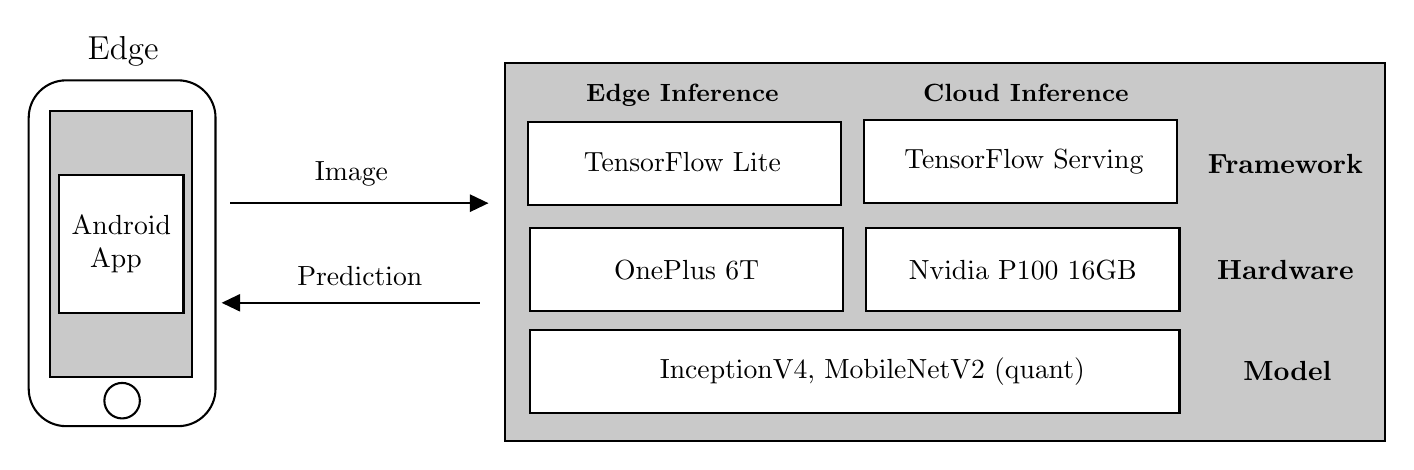
\begin{tikzpicture}[x=0.75pt,y=0.75pt,yscale=-1,xscale=1]
%uncomment if require: \path (0,485.57142639160156); %set diagram left start at 0, and has height of 485.57142639160156

%Straight Lines [id:da9993479608904674] 
\draw    (100.48,89) -- (223,89) ;
\draw [shift={(225,89)}, rotate = 540] [fill={rgb, 255:red, 0; green, 0; blue, 0 }  ][line width=0.75]  [draw opacity=0] (8.93,-4.29) -- (0,0) -- (8.93,4.29) -- cycle    ;

%Straight Lines [id:da5401559459790608] 
\draw    (98.48,137) -- (221,137) ;

\draw [shift={(96.48,137)}, rotate = 360] [fill={rgb, 255:red, 0; green, 0; blue, 0 }  ][line width=0.75]  [draw opacity=0] (8.93,-4.29) -- (0,0) -- (8.93,4.29) -- cycle    ;
%Shape: Rectangle [id:dp45054130026891115] 
\draw  [fill={rgb, 255:red, 201; green, 201; blue, 201 }  ,fill opacity=1 ] (233,21.57) -- (656.93,21.57) -- (656.93,203.57) -- (233,203.57) -- cycle ;
%Shape: Rectangle [id:dp21016153851852382] 
\draw  [fill={rgb, 255:red, 255; green, 255; blue, 255 }  ,fill opacity=1 ] (245,150) -- (557.93,150) -- (557.93,190) -- (245,190) -- cycle ;
%Shape: Rectangle [id:dp17739269402878732] 
\draw  [fill={rgb, 255:red, 255; green, 255; blue, 255 }  ,fill opacity=1 ] (244,50) -- (394.93,50) -- (394.93,90) -- (244,90) -- cycle ;
%Shape: Rectangle [id:dp9093436455970001] 
\draw  [fill={rgb, 255:red, 255; green, 255; blue, 255 }  ,fill opacity=1 ] (406,49) -- (556.93,49) -- (556.93,89) -- (406,89) -- cycle ;
%Shape: Rectangle [id:dp14120602080303146] 
\draw  [fill={rgb, 255:red, 255; green, 255; blue, 255 }  ,fill opacity=1 ] (245,101) -- (395.93,101) -- (395.93,141) -- (245,141) -- cycle ;
%Shape: Rectangle [id:dp45473714544487454] 
\draw  [fill={rgb, 255:red, 255; green, 255; blue, 255 }  ,fill opacity=1 ] (407,101) -- (557.93,101) -- (557.93,141) -- (407,141) -- cycle ;
%Shape: Rectangle [id:dp4153343207585154] 
\draw  [fill={rgb, 255:red, 201; green, 201; blue, 201 }  ,fill opacity=1 ] (13.91,44.69) -- (82.34,44.69) -- (82.34,172.63) -- (13.91,172.63) -- cycle ;
%Rounded Rect [id:dp09380596237315397] 
\draw   (3.5,47.82) .. controls (3.5,37.88) and (11.56,29.82) .. (21.5,29.82) -- (75.5,29.82) .. controls (85.44,29.82) and (93.5,37.88) .. (93.5,47.82) -- (93.5,178.43) .. controls (93.5,188.37) and (85.44,196.43) .. (75.5,196.43) -- (21.5,196.43) .. controls (11.56,196.43) and (3.5,188.37) .. (3.5,178.43) -- cycle ;
%Shape: Ellipse [id:dp8964060056788943] 
\draw   (39.95,184.16) .. controls (39.95,179.43) and (43.78,175.6) .. (48.5,175.6) .. controls (53.22,175.6) and (57.05,179.43) .. (57.05,184.16) .. controls (57.05,188.88) and (53.22,192.71) .. (48.5,192.71) .. controls (43.78,192.71) and (39.95,188.88) .. (39.95,184.16) -- cycle ;
%Shape: Rectangle [id:dp85708751067272] 
\draw  [fill={rgb, 255:red, 255; green, 255; blue, 255 }  ,fill opacity=1 ] (18.19,75.22) -- (78.07,75.22) -- (78.07,142.1) -- (18.19,142.1) -- cycle ;

% Text Node
\draw (159,75) node  [align=left] {Image};
% Text Node
\draw (163,124) node  [align=left] {Prediction};
% Text Node
\draw (49,16) node  [align=left] {{\large Edge}};
% Text Node
\draw (409.96,170) node  [align=left] {InceptionV4, MobileNetV2 (quant)};
% Text Node
\draw (318.46,37) node  [align=left] {{\small \textbf{Edge Inference}}};
% Text Node
\draw (483.96,36) node  [align=left] {{\small \textbf{Cloud Inference}}};
% Text Node
\draw (318.46,69) node  [align=left] {TensorFlow Lite};
% Text Node
\draw (482.96,68.79) node  [align=left] {TensorFlow Serving};
% Text Node
\draw (320.46,121) node  [align=left] {OnePlus 6T};
% Text Node
\draw (482.46,121) node  [align=left] {Nvidia P100 16GB};
% Text Node
\draw (608.96,70) node  [align=left] {\textbf{Framework}};
% Text Node
\draw (608.96,121) node  [align=left] {\textbf{Hardware}};
% Text Node
\draw (609.96,170) node  [align=left] {\textbf{Model}};
% Text Node
\draw (48.13,108.66) node  [align=left] {Android\\ \ \ App};


\end{tikzpicture}